\section{Network-on-chip}
Network-on-chip (NoC) has become a crucial component for data communication in modern processors, offering high throughput, low latency, and efficient power utilization.
The performance of NoCs is influenced by various factors such as topology, routing algorithms, switching mechanisms, and link/channel width.
With the goal in achieving optimal performance, researchers have looked into exploring different aspects of NoC design to enhance its efficiency.
One key element that significantly impacts NoC performance is the choice of topology.
Studies have shown that selecting an appropriate topology is critical as it affects zero-load latency, sustainable bandwidth, and power consumption \cite{chenPhysicalVsVirtual2010}.
For instance, the 2D mesh topology (see \cref{fig:config_noc}), as utilized in the \graicore{}, is commonly used in NoCs due to its scalability and fault tolerance, enabling efficient communication among cores.

% \begin{figure}[htbp]
% \centering
% 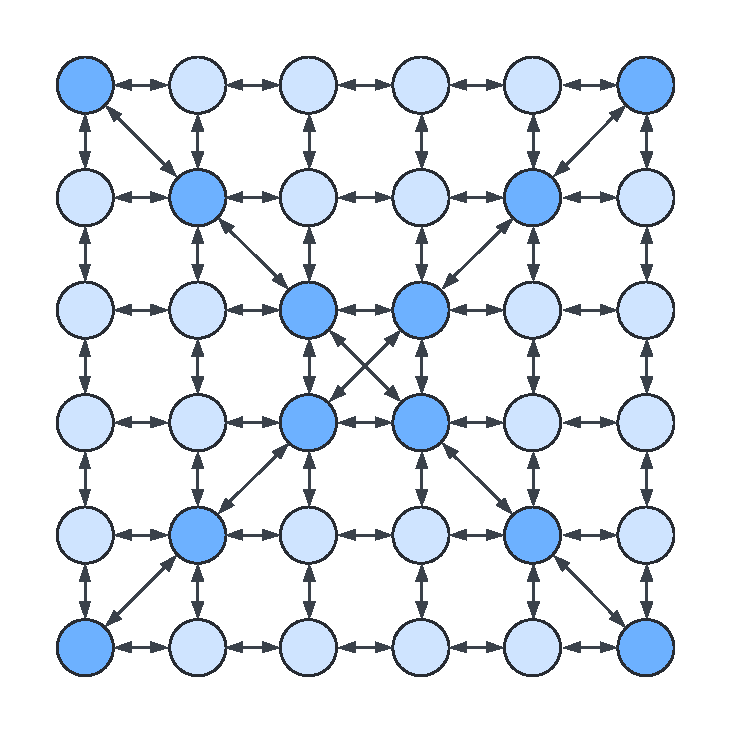
\includegraphics[width=0.45\textwidth]{assets/xdmesh_topology.pdf}
% \caption{
% An 6x6 XDMesh topology.
% The darker blue shaded nodes feature additional diagonal links.
% }
% \label{fig:xdmesh_topology}
% \end{figure}

% Additionally, the extended diagonal mesh (XDMesh) has been proposed as an enhancement to the 2D mesh topology \cite{furhadExtendedDiagonalMesh2015}.
% XDMesh improves the 2D mesh by incorporating diagonal links (see example in \cref{fig:xdmesh_topology}), which decrease the network diameter---the longest distance between two nodes situated at opposite diagonal corners of the 2D mesh.
% This reduction in network diameter leads to lower communication delays and fewer hop counts.
% Experimental results show that XDMesh achieves over $40\%$ better throughput and latency compared to the 2D mesh.
% Furthermore, it outperforms the 2D mesh in terms of energy efficiency, with minimal differences in silicon area.
% The experimental environment makes use of the uniform traffic model, where each node in the network generates and sends data packets to all other nodes with equal probability.
% When transferring data from an external source, data is only injected into \graicore{}'s NoC via a single point.
% For this reason, the employed uniform traffic model is not a representative traffic pattern for the \confignoc{}. 
% However, the relatively small topology change introduced by XDMesh can still be worthwhile to consider for improving NoC's performance.

Routing algorithms play a crucial role in determining the efficiency of data transmission in NoCs.
Research has focused on developing novel routing algorithms to optimize performance.
For example, a study introduced a low-latency routing algorithm that exploits path diversity to achieve high bandwidth and low latency in NoC routers \cite{yangExploitingPathDiversity2012}.
Furthermore, the design of energy-efficient routing algorithms has been explored to enhance the overall power efficiency of NoCs \cite{parikhPowerAwareNoCsRouting2014}.
These routing algorithms aim to balance the trade-off between performance metrics such as throughput and latency while minimizing power consumption.
The current configuration procedure for the \graicore{} transmits data packets from an external source to the destination neuron cores in a sequential manner, utilizing the XY routing algorithm \cite{glassTurnModelAdaptive1992}.
XY routing, being a non-adaptive algorithm, ensures that data packets always traverses the same path from source to destination.
Consequently, the traffic pattern remains straightforward.
At a time, there is only a single flow of data from source to destination.
Because of this, no parallel communication occurs during the configuration process and therefore the congestion is minimal.
However, if we choose to explore a NoC design or configuration procedure that involves concurrent traffic through the network, potential congestion issues may arise.
In such cases, a suitable routing algorithm must be implemented to manage and mitigate congestion effectively.

Switching techniques in NoCs determines how data packets are forwarded within the network, thereby influencing bandwidth, latency and power consumption.
Research has proposed energy-efficient reconfigurable circuit-switched NoCs as a means to optimize power utilization while maintaining high performance \cite{wolkotteEnergyEfficientReconfigurableCircuitSwitched2005}.
Additionally, studies on switching techniques with reduced buffer requirements highlight the importance of balancing performance and power efficiency in modern NoC designs \cite{requenaEfficientSwitchingTechnique2008}.
By implementing efficient switching mechanisms, designers can achieve lower power consumption without compromising network performance.

Link width is another essential design parameter that influences the overall bandwidth of the network.
Wider links can accommodate higher data rates, leading to improved throughput and reduced latency.
However, the use of wider links also consume more power, so there is a trade-off between performance and power consumption that designers need to consider when designing a NoC \cite{manhokimNetworkonchipLinkAnalysis2006}.
Widening the link widths in the \graicore{}'s NoC is a relatively straightforward enhancement, making it an appealing solution for improving both throughput and latency.
However, it is important to note that increasing the link widths also requires more silicon area due to the need for additional physical wires and increased router complexity.

% In conclusion, NoC technology has emerged as a vital component in many-core processors, providing high throughput, low latency, and efficient power utilization.
% The performance of NoCs is shaped by several key factors, including topology, routing algorithms, switching mechanisms, and link width.
% Research has highlighted the importance of selecting the right topology, such as the XDMesh, which can significantly enhance performance by reducing communication delays and hop counts.
% Efficient routing algorithms and switching techniques further optimize data transmission and power efficiency.
% Additionally, adjusting link widths offers a means to improve throughput and latency, though it must be balanced against increased power consumption and silicon area.